% Copyright 2010, Tony R. Kuphaldt, released under the Creative Commons Attribution License (v 1.0)
% This means you may do almost anything with this work of mine, so long as you give me proper credit

To endebrytere skal tilkobles h.h.v. \texttt{DI2} og \texttt{DI5} på en Wago 750-430 DI inngangsmodul. Tegn de nødvendige koblingene. Det internekoblingsskjemaet for (\texttt{DI1}) vises som en referanse for alle inngangene.
Tegn de nødvendige koblingene som er nødvendig for tilkobling av endebryterene.  


$$\includegraphics[width=15.5cm]{i04806x01.eps}$$

Er dette en \textit{sinking} eller en \textit{sourcing} DI modul?

\vskip 20pt \vbox{\hrule \hbox{\strut \vrule{} {\bf Suggestions for Socratic discussion} \vrule} \hrule}

\begin{itemize}
\item{} If you have identified this module as sourcing, explain how its design would differ to make it {\it sinking}.  If you have identified this module as sinking, explain how its design would differ to make it {\it sourcing}.
\item{} Explain how this module's internal circuitry could be modified to allow it to source {\it or} sink current, instead of doing just one of these functions.
\end{itemize}

\underbar{file i04806}
%(END_QUESTION)





%(BEGIN_ANSWER)

This particular input module {\it sinks} current from the limit switches (arrows drawn in the direction of conventional flow):

$$\includegraphics[width=15.5cm]{i04536x02.eps}$$



\vfil \eject



%(END_ANSWER)





%(BEGIN_NOTES)



\noindent
{\bf Prep Quiz:}

The Allen-Bradley MicroLogix 1000 PLC has the ability to either {\it source} or {\it sink} at its DC input terminals.  Determine the direction of current through each limit switch when closed:

$$\includegraphics[width=15.5cm]{i04536x03.eps}$$

Sketch or state your directions of current following {\it conventional flow} notation.




\vfil \eject

\noindent
{\bf Prep Quiz:}

This particular Allen-Bradley MicroLogix 1000 PLC has the ability to either {\it source} or {\it sink} at its relay-contact output terminals.  Determine the direction of current through each lamp when its respective output is activated:

$$\includegraphics[width=15.5cm]{i04536x04.eps}$$

Sketch or state your directions of current following {\it conventional flow} notation.










\vfil \eject

\noindent
{\bf Prep Quiz:}

Identify the stimulus condition of each switch in this PLC system, based on the color highlighting seen in the ladder-logic PLC program:

$$\includegraphics[width=15.5cm]{i04536x05.eps}$$

Level = {\it high} or {\it low}? \hskip 40pt Pressure = {\it high} or {\it low}? \hskip 40pt Flow = {\it high} or {\it low}?









\vfil \eject

\noindent
{\bf Prep Quiz:}

Identify the stimulus condition of each switch in this PLC system, based on the color highlighting seen in the ladder-logic PLC program:

$$\includegraphics[width=15.5cm]{i04536x06.eps}$$

Level = {\it high} or {\it low}? \hskip 40pt Pressure = {\it high} or {\it low}? \hskip 40pt Flow = {\it high} or {\it low}?










\vfil \eject

\noindent
{\bf Prep Quiz:}

Identify the stimulus condition of each switch in this PLC system, based on the color highlighting seen in the ladder-logic PLC program:

$$\includegraphics[width=15.5cm]{i04536x07.eps}$$

Level = {\it high} or {\it low}? \hskip 40pt Pressure = {\it high} or {\it low}? \hskip 40pt Flow = {\it high} or {\it low}?


%INDEX% PLC, I/O: discrete I/O device wiring

%(END_NOTES)


